%%%%%%%%%%%%%%%%%%%%%%%%%%%%%%%%%%%%%%%%%%%%%%%%%%%%%%%%%%%
% Preliminary (beta) report — E-Bike Battery-Swap Network
% Built on the rho-class template (CC BY 4.0, G. Jimenez)
%
% Place the rho-class/ folder, a figures/ folder (with the PNGs from
% data/exports/report and data/exports/sensitivity), and rho.bib next to
% this file. Compile with pdfLaTeX (shell-escape not required if you remove
% the minted listing).
%%%%%%%%%%%%%%%%%%%%%%%%%%%%%%%%%%%%%%%%%%%%%%%%%%%%%%%%%%%

\documentclass[9pt,a4paper,twocolumn,twoside]{rho-class/rho}
\usepackage[english]{babel}

%----------------------------------------------------------
% Title
%----------------------------------------------------------

\doctype{Preliminary Report (Beta)}
\title{A Digital-Twin Simulation and AI Decision-Support System for E-Bike Battery-Swap Locker Networks}

%----------------------------------------------------------
% Authors, Affiliations and dates
%----------------------------------------------------------

\author[{\textasteriskcentered},a,1]{Louis Battle}

\affil[a]{E-Bike Battery-Swap Network Simulation Project}

\dates{Preliminary beta report, compiled \today}

%----------------------------------------------------------
% Corresponding author / document info
%----------------------------------------------------------

\corres{\textsuperscript{\textasteriskcentered}Corresponding author.}

\docinfo{This is a preliminary (beta) report. All simulation parameters are
documented best-estimates pending real operator data; results are therefore
to be read as \emph{relative} and \emph{structural} rather than absolute
predictions.}

%----------------------------------------------------------

\journalname{E-Bike Battery-Swap Network Simulation}
\journal{Beta Report}
\theday{\today}
\vol{1}
\no{1}

%----------------------------------------------------------
% Abstract and Keywords
%----------------------------------------------------------

\begin{abstract}
    Urban e-bike delivery is creating fast-growing demand for battery-swap
    locker infrastructure, yet deciding \emph{where}, \emph{how many}, and
    \emph{what size} lockers to deploy is largely intuition-driven and
    expensive to test in the field. We present a digital-twin, agent-based
    simulation of a battery-swap network built on the real Amsterdam street
    network, together with an end-to-end machine-learning pipeline that learns
    from the simulator and recommends locker placement. The simulation models
    riders, battery physics in watt-hours, demand hotspots, locker inventory
    and charging, weather, and route constraints such as ferry crossings. A
    sensitivity analysis confirms the model responds correctly to its inputs.
    A gradient-boosted surrogate trained on 500 simulated scenarios predicts
    key outcomes accurately (mean stranded riders: $R^2=0.96$, Spearman
    $0.98$), and a greedy optimiser using this surrogate produces locker
    placements that reduce stranded riders by $\sim$20\% versus random
    placement at an equal budget. We report the system architecture,
    validation, results, and a roadmap toward operator-data calibration.
\end{abstract}

\keywords{Agent-based simulation, Digital twin, Battery swapping, Facility
location, Surrogate modelling, Gradient boosting, Urban mobility}

%----------------------------------------------------------

\begin{document}

    \maketitle
    \thispagestyle{firststyle}
    \tableofcontents

%----------------------------------------------------------

\section{Introduction}

    \rhostart{U}rban e-bike delivery services depend on a reliable supply of
    charged batteries. Battery-swap operators provide networks of physical
    lockers where riders exchange a depleted battery for a charged one. For
    such an operator, the central planning questions are expensive and
    high-stakes: \emph{where} should lockers be installed, \emph{how many} are
    needed for a given level of demand, and \emph{what capacity} each location
    requires. Testing these decisions in the field disrupts operations and is
    costly.

    This project develops a \emph{digital twin}: a simulation that reproduces
    the relevant dynamics of a swap network in a real city, plus an
    AI layer that learns from the simulation to recommend infrastructure
    decisions. This document reports the beta state of the system. Because the
    simulator is currently calibrated on documented best-estimates rather than
    operator data, results are presented as relative and structural; the
    architecture is designed so that real data can be substituted and the
    models retrained without redesign.

\section{Simulation Engine}

    The simulator is agent-based \cite{mesa2020} and organised in layers, each
    corresponding to a real-world planning concern.

    \begin{itemize}
        \item \textbf{City graph.} The Amsterdam bike network from
        OpenStreetMap via OSMnx \cite{boeing2017osmnx}, where nodes are
        intersections and edges are streets with real lengths; routing uses
        NetworkX \cite{hagberg2008networkx}. The graph is restricted to its largest strongly connected
        component so every location is reachable.
        \item \textbf{Riders.} Agents that travel shortest (fastest) paths,
        consume battery in proportion to distance, seek a locker when low, and
        strand if depleted.
        \item \textbf{Demand.} Weighted hotspot zones (city centre, dining
        districts, stations) that drive where deliveries originate and end.
        \item \textbf{Lockers.} Finite-capacity stations (7, 8, or 10 slots)
        with time-based charging of returned batteries.
        \item \textbf{Conditions.} Weather (rain, wind, snow, heat) scales
        riding speed and battery drain; route constraints include the
        Centraal--Noord ferry.
    \end{itemize}

    \subsection{Physical battery model}

        Battery state is tracked in watt-hours so values are checkable against
        real specifications. With capacity $C$ (Wh) and consumption $c$
        (Wh/km), the full range is given by \equref{eq:range}.

        \begin{equation}\label{eq:range}
            R = \frac{C}{c}
        \end{equation}

        The beta uses $C=500$~Wh and $c=12$~Wh/km, giving $R \approx 42$~km
        (about 33~km to the 20\% reserve threshold). Edge travel time follows
        $t = \ell / v$ for edge length $\ell$ and speed $v$; weather multiplies
        both travel time and battery cost.

\section{Calibration}

    All physical and behavioural parameters are documented best-estimates
    pending operator data (\tabref{tab:params}). They produce
    directionally-correct behaviour but are not yet validated for absolute
    accuracy. The architecture isolates these values in configuration so that
    real measurements can replace them and the pipeline can be re-run.

    \begin{table}[H]
        \caption{Key beta parameters (best estimates).}
        \label{tab:params}
        \begin{tabular}{
            >{\raggedright\arraybackslash}p{0.45\columnwidth}
            >{\raggedright\arraybackslash}p{0.40\columnwidth}
        }
        \toprule
        \textbf{Parameter} & \textbf{Value} \\
        \midrule
        Battery capacity & 500 Wh \\
        Energy consumption & 12 Wh/km \\
        Reserve threshold & 20\% \\
        Rider speed & 18 km/h \\
        Charge time (per battery) & 3.5 h \\
        Locker capacities & 7 / 8 / 10 slots \\
        Time step & 10 s \\
        \bottomrule
        \end{tabular}
        \tabletext{Note: see the project calibration document for the basis and
        confidence level of each value.}
    \end{table}

\section{Validation and Sensitivity Analysis}

    Before any learning, a one-at-a-time sensitivity analysis confirms the
    simulator responds in the correct direction and magnitude.
    \figref{fig:tornado} ranks parameter impact on service failures. The key
    findings: adding lockers reduces stranded riders and raises swap-success
    rate; increasing rider count raises throughput but also strandings;
    worsening weather reduces throughput. Impact on strandings ranks as
    \emph{demand} $\gg$ \emph{locker count} $>$ \emph{speed} $>$ \emph{weather}
    --- i.e.\ the two business levers (demand load and supply) are correctly
    dominant.

    \begin{figure}[H]
        \centering
        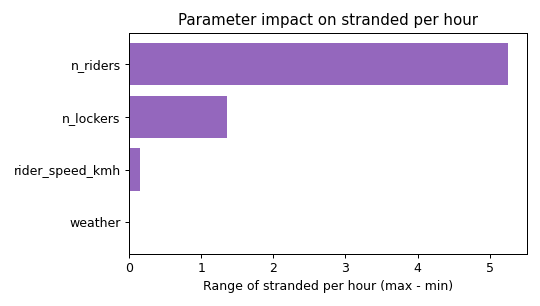
\includegraphics[width=0.95\columnwidth]{figures/tornado.png}
        \caption{Parameter impact on stranded riders per hour (range of the
        mean across each parameter's swept values).}
        \label{fig:tornado}
    \end{figure}

\section{Experiment Framework and Data Generation}

    A reproducible experiment framework turns the simulator into a training
    dataset. Candidate locker sites are generated from demand hotspots plus
    farthest-point spread. A sampler draws random combinations of
    \emph{layout} (a subset of candidate sites) and \emph{scenario} (rider
    count, weather, speed); a driver runs each to steady state and records one
    row of engineered features and outcome metrics. The graph is loaded once
    and runs execute in parallel across CPU cores. For this report, 500
    scenarios were generated on the Amsterdam network.

    Each row's \emph{features} describe the layout's relationship to demand
    (coverage within travel-time thresholds, demand-weighted distance to the
    nearest locker, dispersion, supply ratios) plus the scenario conditions.
    The \emph{targets} are normalised, steady-state outcome metrics (stranded
    riders, swap-success rate, throughput, locker utilisation, battery level).

\section{AI Decision-Support}

    The AI is two distinct components separated by the dataset: a
    \emph{surrogate} that learns outcomes, and an \emph{optimiser} that searches
    placements using the surrogate.

    \subsection{Surrogate model}

        A multi-output gradient-boosted regressor (one model per target,
        scikit-learn \cite{scikit-learn}) maps features to outcomes. Evaluation uses a group-wise train/test split
        (replicate seeds never cross the split). \figref{fig:accuracy} and
        \figref{fig:parity} show accuracy by target. Outcomes that vary smoothly
        with demand and supply are predicted very well (mean stranded riders
        $R^2=0.96$, battery $0.92$, throughput $0.81$); noisy failure-\emph{rate}
        metrics are only moderately predictable ($R^2\approx0.5$).

        \begin{figure}[H]
            \centering
            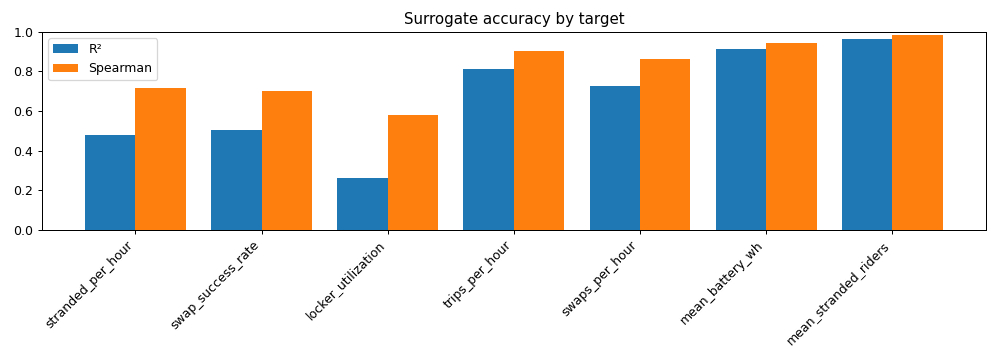
\includegraphics[width=0.95\columnwidth]{figures/surrogate_accuracy.png}
            \caption{Surrogate accuracy ($R^2$ and Spearman rank correlation)
            per target on the held-out test set.}
            \label{fig:accuracy}
        \end{figure}

        \begin{figure}[H]
            \centering
            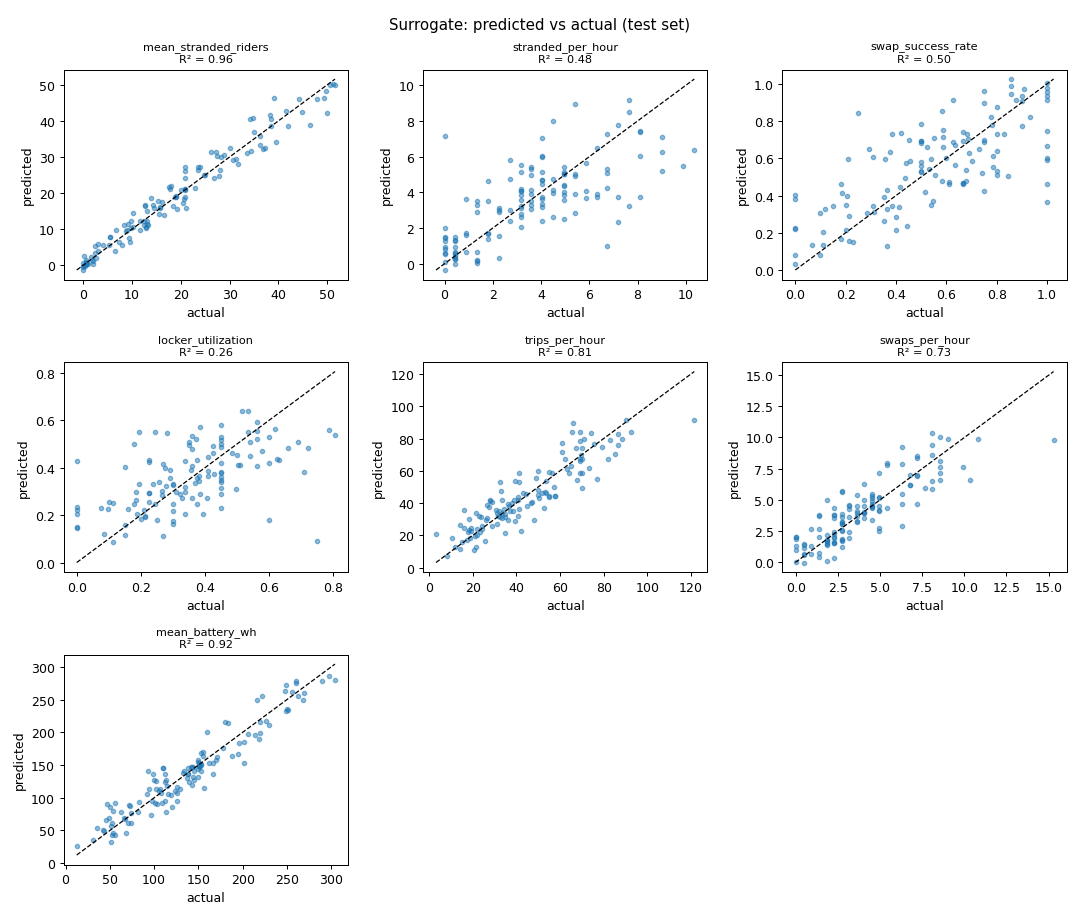
\includegraphics[width=0.95\columnwidth]{figures/surrogate_parity.png}
            \caption{Predicted versus actual values on the test set; the dashed
            line is perfect prediction.}
            \label{fig:parity}
        \end{figure}

        Permutation feature importance (\figref{fig:importance}) shows that
        stranded riders are driven primarily by rider count and the
        lockers-per-rider ratio, with spatial features contributing a smaller
        share --- the model is strongest at network \emph{sizing}.

        \begin{figure}[H]
            \centering
            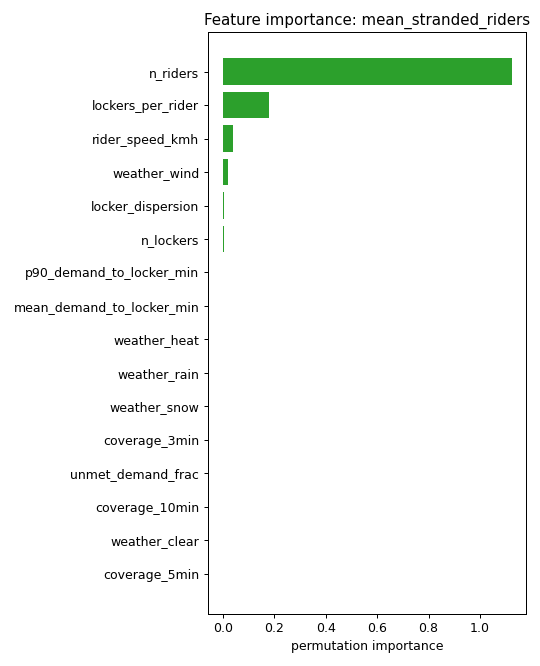
\includegraphics[width=0.95\columnwidth]{figures/feature_importance.png}
            \caption{Permutation feature importance for mean stranded riders.}
            \label{fig:importance}
        \end{figure}

    \subsection{Objective and optimiser}

        Candidate placements are scored by a single objective combining the
        well-predicted, non-degenerate service signal (mean stranded riders,
        minimised) with optional secondary terms. Each target is normalised to
        $[0,1]$ and minimisation targets are flipped, giving the weighted score
        in \equref{eq:objective}, where $g_t$ is the normalised, direction-
        adjusted value of predicted target $\hat{y}_t$ and $w_t$ its weight.

        \begin{equation}\label{eq:objective}
            S(\hat{y}) = \frac{1}{\sum_t w_t}\sum_t w_t\, g_t(\hat{y}_t)
        \end{equation}

        A forward-greedy optimiser repeatedly adds the candidate site that most
        improves $S$, producing both a recommended layout and the full
        score-versus-budget curve.

\section{Results}

    \figref{fig:curve} shows the objective rising with the number of lockers and
    plateauing --- a clear diminishing-returns curve that answers ``how many
    lockers''. To test placement \emph{quality} at a fixed budget, we compared
    the optimiser's six-locker recommendation against random six-locker layouts,
    averaged over three seeds to suppress run-to-run noise
    (\figref{fig:comparison}). The optimised placement yields 14.96 mean
    stranded riders versus 18.72 for random --- a $\sim$20\% reduction, and it
    beats every random layout tested. \tabref{tab:results} summarises the
    headline metrics.

    \begin{figure}[H]
        \centering
        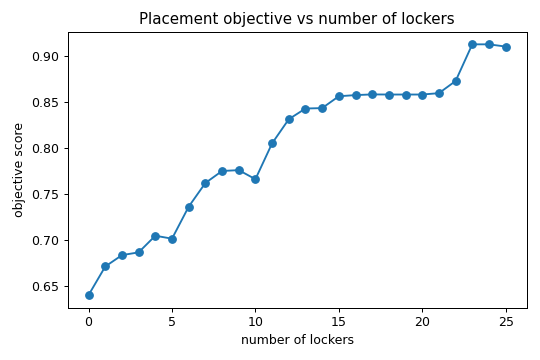
\includegraphics[width=0.9\columnwidth]{figures/optimization_curve.png}
        \caption{Objective score versus number of lockers (greedy placement).}
        \label{fig:curve}
    \end{figure}

    \begin{figure}[H]
        \centering
        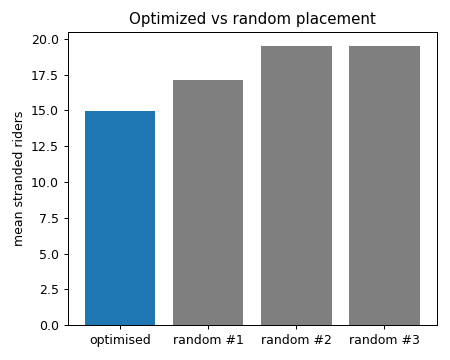
\includegraphics[width=0.8\columnwidth]{figures/placement_comparison.png}
        \caption{Optimised versus random placement at a six-locker budget
        (mean stranded riders, seed-averaged).}
        \label{fig:comparison}
    \end{figure}

    \begin{table}[H]
        \caption{Headline beta results.}
        \label{tab:results}
        \begin{tabular}{
            >{\raggedright\arraybackslash}p{0.55\columnwidth}
            >{\raggedright\arraybackslash}p{0.30\columnwidth}
        }
        \toprule
        \textbf{Result} & \textbf{Value} \\
        \midrule
        Surrogate $R^2$ (mean stranded riders) & 0.96 \\
        Surrogate Spearman (mean stranded) & 0.98 \\
        Training scenarios & 500 \\
        Placement improvement vs random & $\sim$20\% \\
        Automated tests passing & 121 \\
        \bottomrule
        \end{tabular}
    \end{table}

\section{Discussion and Limitations}

    The pipeline works end-to-end and the closing-the-loop verification (running
    the recommended layout back through the simulator) confirms a genuine
    placement gain. Two qualifications are important. First, the system is
    calibrated on estimates, so results are relative, not absolute predictions.
    Second, the surrogate is strongest at \emph{sizing} the network; the spatial
    signal that distinguishes good from bad \emph{placement} is real but
    secondary, so the placement advantage is clearest at constrained budgets and
    must be measured with seed averaging. These are properties of the current
    data and metrics, not flaws in the architecture.

\section{Future Work}

    Priorities for the next iteration: (i) obtain operator data (battery specs,
    fleet/demand figures, candidate sites, service-level targets) to calibrate
    and validate against real KPIs; (ii) strengthen the placement signal through
    more data, seed-replicated denoising, and richer spatial features; (iii) add
    locker capacity as a decision variable; and (iv) move toward a spatial
    (raster/CNN) representation enabling per-city ``suitability heatmaps'' for
    pre-deployment planning in new cities.

\section{Conclusion}

    We have built and validated a digital-twin simulation of an e-bike
    battery-swap network and an AI pipeline that learns from it to recommend
    locker placement. On estimate-calibrated data the surrogate predicts the
    key service metric with high accuracy and the optimiser reduces stranded
    riders by roughly 20\% versus random placement. The result is a credible
    beta and a clear path to an operator-calibrated decision-support tool.

%----------------------------------------------------------

\printbibliography

%----------------------------------------------------------

\end{document}
